\documentclass[12pt]{article}

% ---- Packages ----
\usepackage[a4paper,margin=1in]{geometry}
\usepackage{setspace}
\usepackage{graphicx}
\usepackage{svg} % requires inkscape; see compile note
\usepackage{float}
\usepackage{booktabs}
\usepackage{longtable}
\usepackage{listings}
\usepackage{xcolor}
\usepackage{amsmath}
\usepackage{amssymb}
\usepackage{hyperref}
\usepackage{makeidx}
\usepackage{tikz}
\usetikzlibrary{positioning,arrows.meta,fit,shapes.geometric,trees}

% Avoid LaTeX text overlays from SVGs to prevent Unicode issues
\svgsetup{inkscapelatex=false}
% ---- Color palette for diagrams ----
\definecolor{eduBlue}{HTML}{1F4E79}
\definecolor{eduCyan}{HTML}{2A9D8F}
\definecolor{eduGreen}{HTML}{2E7D32}
\definecolor{eduOrange}{HTML}{F4A261}
\definecolor{eduRed}{HTML}{E76F51}
\definecolor{eduGray}{HTML}{F2F2F2}

\tikzset{
  block/.style={draw, rounded corners, fill=eduGray, minimum width=3.4cm, minimum height=1cm, font=\small},
  blockBlue/.style={block, fill=eduBlue!15, draw=eduBlue},
  blockCyan/.style={block, fill=eduCyan!15, draw=eduCyan},
  blockGreen/.style={block, fill=eduGreen!15, draw=eduGreen},
  blockOrange/.style={block, fill=eduOrange!18, draw=eduOrange},
  blockRed/.style={block, fill=eduRed!18, draw=eduRed},
  arrow/.style={-{Latex}, line width=0.6pt, shorten >=2pt, shorten <=2pt},
  edgeLabel/.style={fill=white, inner sep=1pt, font=\scriptsize, align=center, yshift=2pt}
}

\hypersetup{colorlinks=true,linkcolor=black,urlcolor=blue,citecolor=black}
\onehalfspacing

\lstset{
  basicstyle=\ttfamily\small,
  breaklines=true,
  frame=single,
  columns=fullflexible
}

\makeindex

\title{\textbf{CSE 3206 Reflection Essay} \\[0.5cm] EduPredict -- AI Student Performance Predictor}
\author{\textbf{Submitted by}\\\textbf{Mashfiq Ahmed Naushad}\\Roll: 2103056\\\\[0.6cm]
\textbf{Submitted to}\\\textbf{Farjana Parvin}\\Assistant Professor\\Dept. of Computer Science \& Engineering, RUET}

\date{February 9, 2026}

\begin{document}
\maketitle
\vspace{1.2cm}
\begin{abstract}
This reflection analyzes my self-directed learning in the EduPredict project, a full-stack system that predicts student risk and provides explainable results to teachers, students, and administrators. The central technical decision was to integrate SHAP explainability with a LightGBM classifier inside a simple ensemble, and to expose explanations through an API. I justify this decision by linking model behavior to stakeholder requirements, code structure, latency constraints, and data governance. I also compare the choice against alternatives with respect to scalability, interpretability, and operational cost. Finally, I evaluate my learning process and present a concrete next-step plan for lifelong professional growth through MLOps practices.
\end{abstract}
\newpage
\tableofcontents
\newpage


\section{Project Context and Scope}
EduPredict is a web application that predicts whether a student is \textit{At-Risk} or \textit{Not-At-Risk} based on academic indicators such as attendance, assignments, quizzes, exams, and GPA. The system supports role-based use cases: administrators manage users, teachers submit and review records, and students view their own outcomes. The system consists of:
\begin{itemize}
  \item A Next.js frontend with role-based dashboards.
  \item A FastAPI backend providing authentication, academic data management, and ML inference.
  \item A database layer (SQLite for local development, PostgreSQL for production).
\end{itemize}

The project required the integration of modern web engineering practices with machine learning inference and explainability. The most significant new technique I independently learned and applied was SHAP-based explainability for tree models, because the problem domain requires transparent decisions and actionable feedback grounded in interpretable evidence.

\subsection{Stack Overview}
The project integrates multiple tools and techniques:
\begin{itemize}
  \item \textbf{Frontend:} Next.js, TypeScript, Tailwind CSS, and charting for dashboards.
  \item \textbf{Backend:} FastAPI, SQLAlchemy, Alembic migrations, and JWT-based RBAC.
  \item \textbf{ML:} scikit-learn for baseline modeling, LightGBM for non-linear modeling, SHAP for explanation, Joblib for artifact storage.
  \item \textbf{Deployment:} Docker for backend packaging and PostgreSQL via Docker Compose.
\end{itemize}

\section{Technical Decision and Justification}
This section provides a deep technical defense of the chosen technique, demonstrating its fit with system constraints, code structure, and operational requirements.

\subsection{Chosen Technique: SHAP for Local Explanations}
I integrated SHAP (SHapley Additive exPlanations) to provide local, per-student explanations. In EduPredict, prediction accuracy alone is insufficient: teachers must understand \textit{why} a student is flagged at risk to plan interventions. SHAP supports this by decomposing a prediction into feature contributions. This is a stronger fit than global feature importance because educators need individualized explanations to choose actions like tutoring, counseling, or academic follow-up.

For a model output $f(x)$, SHAP represents the prediction as:
{\large
\begin{equation}
  f(x) = \phi_0 + \sum_{i=1}^{n} \phi_i,
\end{equation}
}
where $\phi_0$ is the expected output and $\phi_i$ is the contribution of feature $i$ for the specific input $x$. This formulation aligns with transparency requirements in educational contexts.

\subsection{Model Choice and Ensemble Rationale}
The inference pipeline uses a simple ensemble of Logistic Regression and LightGBM. The final probability is the mean of the two model probabilities:
{\large
\begin{equation}
  p = \frac{1}{2}p_{\text{LR}} + \frac{1}{2}p_{\text{LGBM}}.
\end{equation}
}
The predicted label is computed with a threshold:
{\large
\begin{equation}
  \hat{y} = \mathbb{1}[p \ge 0.5].
\end{equation}
}

Logistic Regression provides a stable baseline and interpretable global trends, while LightGBM captures non-linear interactions common in academic performance data (e.g., high GPA with low attendance). SHAP TreeExplainer is optimized for tree models, making LightGBM the most practical choice for efficient, consistent explanations. From a code-structure perspective, the backend isolates ML logic in a dedicated ML module, so the ensemble and explanation logic are encapsulated away from API routing and data access layers, which keeps concerns separated and testing feasible.

\subsection{Scalability and Memory Considerations}
The explanation path must be efficient because it runs alongside API requests. TreeExplainer for LightGBM executes in $O(T\cdot L)$ where $T$ is the number of trees and $L$ is the maximum depth, which is significantly more efficient than kernel-based explainers that scale with the number of samples and features. This makes SHAP feasible for real-time use. In memory terms, the LightGBM model is compact relative to neural alternatives and can be loaded once and cached in the inference process.

\subsection{Comparison with Alternatives}
I considered two alternatives:
\begin{itemize}
  \item \textbf{Pure Logistic Regression with coefficient explanations.} This option is globally interpretable but underfit the data; it missed non-linear patterns and produced weaker predictive performance.
  \item \textbf{LIME or permutation feature importance.} LIME provides local explanations but is stochastic and slower for real-time APIs. Permutation importance is global and does not explain individual predictions. In contrast, SHAP with TreeExplainer provides consistent local explanations with lower latency.
\end{itemize}

The SHAP + LightGBM choice was more effective because it balanced predictive accuracy with stakeholder-facing transparency, and it integrated efficiently into the API. It also supported a clean code separation: the model registry stores artifacts, inference loads the latest model once, and the API layer returns both prediction and explanation.

\subsection{Technical Defense Summary}
The chosen technique satisfied the following constraints simultaneously:
\begin{itemize}
  \item \textbf{Interpretability:} local explanations for each student using SHAP.
  \item \textbf{Performance:} efficient tree-based explanation with predictable latency.
  \item \textbf{Maintainability:} isolated ML module, registry-based versioning, and minimal coupling with API routing.
  \item \textbf{Scalability:} compatible with CPU-only environments and lightweight container deployment.
\end{itemize}

\section{Self-Directed Learning Experience}
\subsection{Key Challenges}
\begin{enumerate}
  \item \textbf{Correct interpretation of SHAP values.} I initially treated SHAP as simple feature importance. I had to learn the distinction between global importance and local contribution and how the baseline affects interpretation.
  \item \textbf{Maintaining feature consistency.} Explanations are only valid if the inference feature order and preprocessing match the training pipeline exactly. I enforced a stable feature list and consistent preprocessing steps in both training and inference paths.
  \item \textbf{Binary classification output formats.} TreeExplainer can return different shapes for binary tasks. I had to identify the correct class-specific SHAP array to avoid incorrect explanations.
  \item \textbf{Asynchronous backend integration.} The backend uses async database sessions and dependency injection. I had to ensure inference and explanation logic did not block the event loop and that model loading was cached properly.
  \item \textbf{Auth and RBAC design.} JWT-based RBAC required careful role checks in API routes so that students only access their own records while admins have broader permissions.
\end{enumerate}

\subsection{Learning Resources and Critical Evaluation}
\begin{longtable}{p{4.2cm}p{5.5cm}p{5.0cm}}
\toprule
\textbf{Resource Type} & \textbf{Strengths} & \textbf{Limitations} \\ \midrule
Official documentation (SHAP, LightGBM, scikit-learn) & Precise definitions, official examples, and correct output formats for explainers. & Dense and time-consuming; assumes prior familiarity with tree-based learning. \\
Tutorials and blog posts & Quick start with runnable code and intuition. & Often omit edge cases, output-shape details, or correct interpretation boundaries. \\
Community forums and GitHub issues & Practical fixes for errors and version-specific quirks. & Inconsistent quality and sometimes outdated or contradictory. \\
\bottomrule
\end{longtable}

Overall, official documentation was the most effective for correctness, while community posts were helpful for specific troubleshooting and error resolution.

\subsection{Self-Assessment of Learning Outcomes}
This experience improved my ability to (1) test assumptions with small experiments, (2) map tool choice to system constraints, and (3) separate concerns in code so ML logic, API routing, and persistence evolve independently. I also gained confidence in reading technical documentation critically rather than using it as a checklist.
\newpage

\section{Project Blocks and Structure}
This section summarizes the project blocks derived from the repository structure and adds additional diagrams to clarify data flow, request lifecycle, and deployment boundaries.

\subsection{Repository-Level Blocks}
\begin{longtable}{ll}
\toprule
\textbf{Block} & \textbf{Responsibility} \\ \midrule
Frontend (apps/frontend) & Next.js UI, dashboards, role-based views, charts \\ 
Backend (apps/backend) & FastAPI API, authentication, ML inference, RBAC \\ 
Database & SQLite for local dev, PostgreSQL via Docker \\ 
ML Registry & Stored model artifacts and metadata \\ 
\bottomrule
\end{longtable}

\subsection{High-Level Architecture Diagram}
\begin{figure}[H]
  \centering
  \includesvg[width=1\textwidth]{figures/Figure_1_High_Level_Architecture}
  \caption{High-level system architecture (from project assets).}
\end{figure}

\subsection{Module Interaction Diagram}
\begin{figure}[H]
  \centering
  \includesvg[width=1\textwidth]{figures/Figure_2_Module_Interaction}
  \caption{Module interaction overview (from project assets).}
\end{figure}

\subsection{Database ER Diagram}
\begin{figure}[H]
  \centering
  \includesvg[width=0.90\textwidth]{figures/Figure_3_Database_ER_Diagram}
  \caption{Database ER diagram (from project assets).}
\end{figure}

\subsection{Explainability Screen}
\begin{figure}[H]
  \centering
  \includesvg[width=0.90\textwidth]{figures/Figure_4_Sample_Prediction_Explanation_Screen}
  \caption{Sample explanation UI (from project assets).}
\end{figure}

\subsection{Product Tour Screens}
\begin{figure}[H]
  \centering
  \includesvg[width=0.8\textwidth]{apps/frontend/public/tour/01-concept}
  \caption{Product concept overview (from project assets).}
\end{figure}

\begin{figure}[H]
  \centering
  \includesvg[width=0.9\textwidth]{apps/frontend/public/tour/02-data-flow}

  \vspace{0.6cm}
  \includesvg[width=0.9\textwidth]{apps/frontend/public/tour/03-explainability}

  \vspace{0.6cm}
  \includesvg[width=0.9\textwidth]{apps/frontend/public/tour/04-interventions}
  \caption{Product tour screens: Data Flow, Explainability, and Intervention Guidance.}
\end{figure}

\subsection{Supplementary Architecture Diagram}
\begin{figure}[H]
\centering
\resizebox{\textwidth}{!}{%
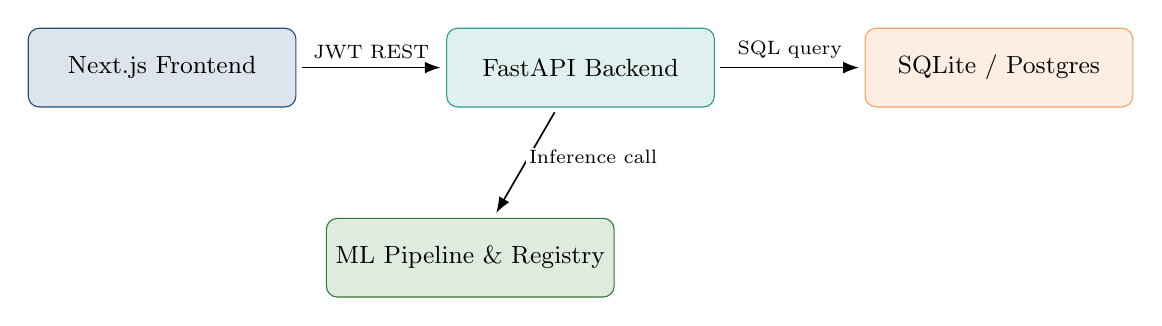
\begin{tikzpicture}[node distance=1.9cm, font=\small]
  \node[blockBlue] (ui) {Next.js Frontend};
  \node[blockCyan, right=of ui] (api) {FastAPI Backend};
  \node[blockOrange, right=of api] (db) {SQLite / Postgres};
  \node[blockGreen, below=1.4cm of api, xshift=-1.4cm] (ml) {ML Pipeline \& Registry};

  \draw[arrow] (ui) -- node[pos=0.5, above, sloped, edgeLabel]{JWT REST} (api);
  \draw[arrow] (api) -- node[pos=0.5, above, sloped, edgeLabel]{SQL query} (db);
  \draw[arrow] (api) -- node[pos=0.5, right, edgeLabel, yshift=0pt]{Inference call} (ml);
\end{tikzpicture}
}
\caption{Supplementary architecture block diagram.}
\end{figure}

\subsection{Prediction Request Sequence}
\begin{figure}[H]
\centering
\resizebox{0.98\textwidth}{!}{%
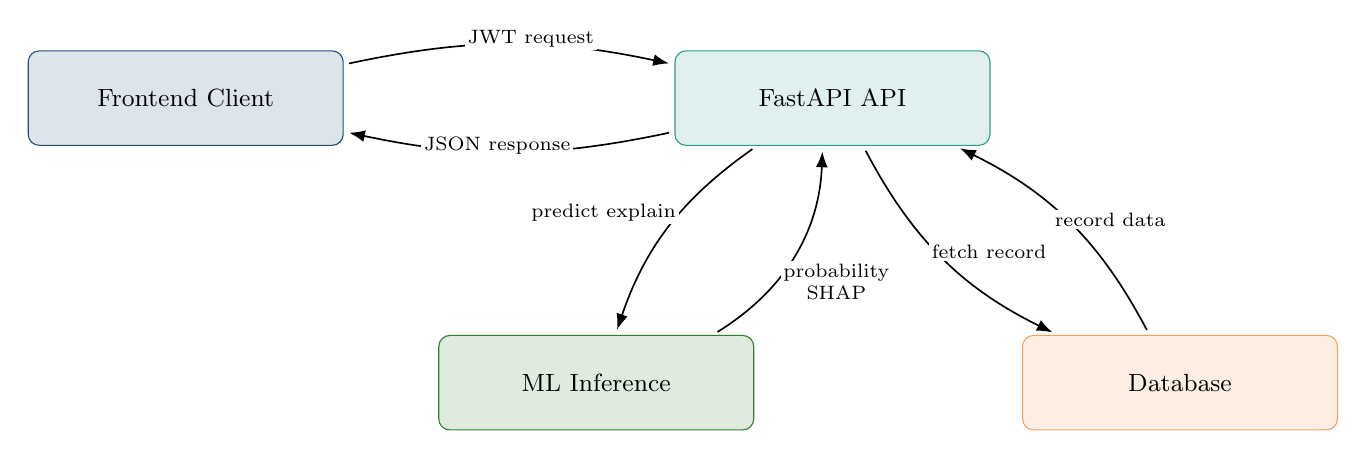
\begin{tikzpicture}[node distance=2.0cm, font=\normalsize]
  \node[blockBlue, minimum width=4.0cm, minimum height=1.2cm] (client) {Frontend Client};
  \node[blockCyan, right=4.2cm of client, minimum width=4.0cm, minimum height=1.2cm] (api) {FastAPI API};
  \node[blockGreen, below=2.4cm of api, xshift=-3.0cm, minimum width=4.0cm, minimum height=1.2cm] (ml) {ML Inference};
  \node[blockOrange, right=4.2cm of ml, xshift=-0.8cm, minimum width=4.0cm, minimum height=1.2cm] (db) {Database};

  \draw[arrow] (client) to[bend left=12] node[pos=0.5, left, edgeLabel, xshift=32pt]{JWT request} (api);
  \draw[arrow] (api) to[bend right=18] node[pos=0.35, left, edgeLabel, xshift=-4pt, yshift=-6pt]{predict explain} (ml);
  \draw[arrow] (ml) to[bend right=28] node[pos=0.65, right, edgeLabel, xshift=-10pt, yshift=-22pt]{probability\\SHAP} (api);
  \draw[arrow] (api) to[bend right=18] node[pos=0.35, right, edgeLabel, xshift=4pt, yshift=-10pt]{fetch record} (db);
  \draw[arrow] (db) to[bend right=18] node[pos=0.65, right, edgeLabel, xshift=4pt, yshift=-10pt]{record data} (api);
  \draw[arrow] (api) to[bend left=12] node[pos=0.5, right, edgeLabel, xshift=-32pt]{JSON response} (client);
\end{tikzpicture}
}
\caption{Sequence of a prediction request with explanation payload.}
\end{figure}

\subsection{ML Training and Registry Flow}
\begin{figure}[H]
\centering
\resizebox{0.98\textwidth}{!}{%
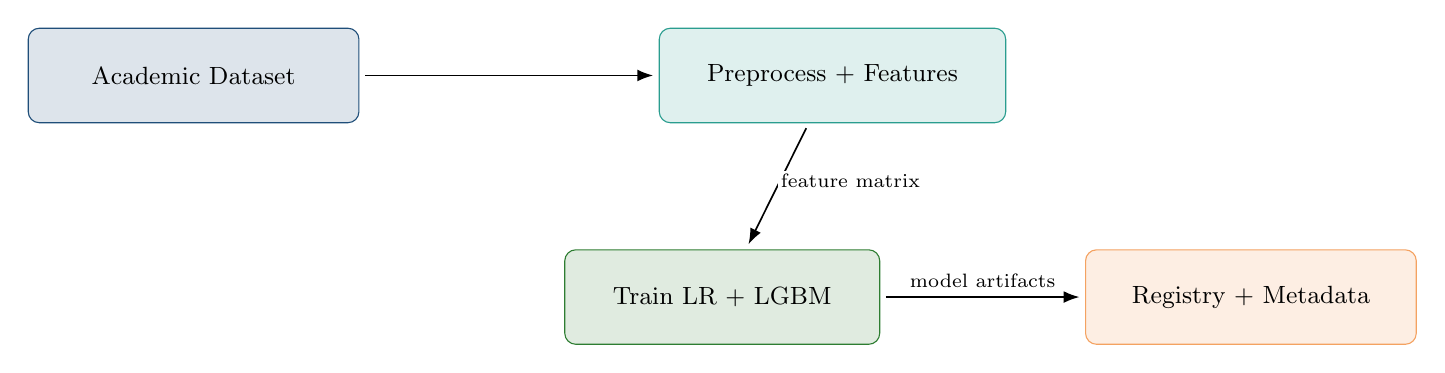
\begin{tikzpicture}[node distance=2.0cm, font=\normalsize]
  \node[blockBlue, minimum width=4.2cm, minimum height=1.2cm] (data) {Academic Dataset};
  \node[blockCyan, right=3.8cm of data, minimum width=4.4cm, minimum height=1.2cm] (prep) {Preprocess + Features};
  \node[blockGreen, below=1.6cm of prep, xshift=-1.4cm, minimum width=4.0cm, minimum height=1.2cm] (train) {Train LR + LGBM};
  \node[blockOrange, right=4.0cm of train, xshift=-1.4cm, minimum width=4.2cm, minimum height=1.2cm] (reg) {Registry + Metadata};

  \draw[arrow] (data) -- (prep);
  \draw[arrow] (prep) -- node[pos=0.5, right, edgeLabel, yshift=0pt]{feature matrix} (train);
  \draw[arrow] (train) -- node[pos=0.5, above, sloped, edgeLabel]{model artifacts} (reg);
\end{tikzpicture}
}
\caption{Training and model registry flow used in EduPredict.}
\end{figure}

\subsection{Deployment Boundary Diagram}
\begin{figure}[H]
\centering
\resizebox{0.98\textwidth}{!}{%
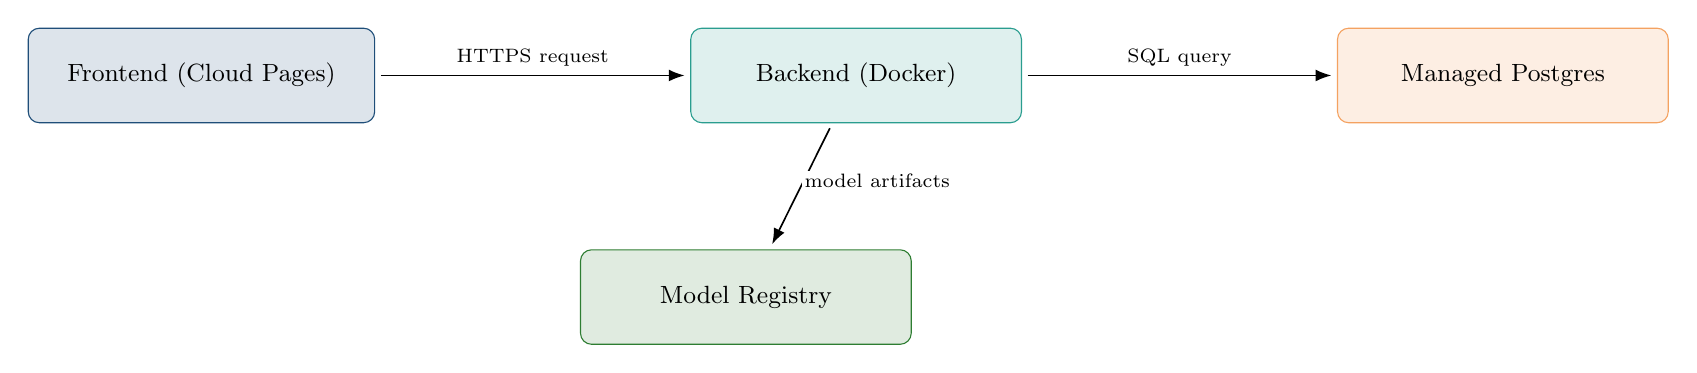
\begin{tikzpicture}[node distance=2.0cm, font=\normalsize]
  \node[blockBlue, minimum width=4.4cm, minimum height=1.2cm] (ui) {Frontend (Cloud Pages)};
  \node[blockCyan, right=4.0cm of ui, minimum width=4.2cm, minimum height=1.2cm] (api) {Backend (Docker)};
  \node[blockOrange, right=4.0cm of api, minimum width=4.2cm, minimum height=1.2cm] (db) {Managed Postgres};
  \node[blockGreen, below=1.6cm of api, xshift=-1.4cm, minimum width=4.2cm, minimum height=1.2cm] (reg) {Model Registry};
  \draw[arrow] (ui) -- node[pos=0.5, above, sloped, edgeLabel]{HTTPS request} (api);
  \draw[arrow] (api) -- node[pos=0.5, above, sloped, edgeLabel]{SQL query} (db);
  \draw[arrow] (api) -- node[pos=0.5, right, edgeLabel, yshift=0pt]{model artifacts} (reg);
\end{tikzpicture}
}
\caption{Deployment boundaries and data flows across services.}
\end{figure}

\subsection{UML-Style Domain Diagram}
\begin{figure}[H]
\centering
\resizebox{0.98\textwidth}{!}{%
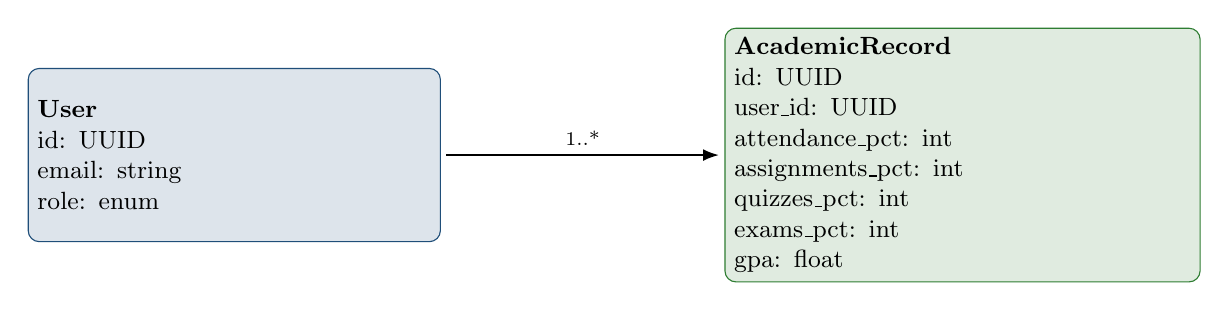
\begin{tikzpicture}[node distance=3.6cm, font=\normalsize]
  \node[blockBlue, minimum width=5.0cm, minimum height=2.2cm, align=left, text width=5.0cm, font=\small] (user) {
    \textbf{User}\\
    id: UUID\\
    email: string\\
    role: enum
  };
  \node[blockGreen, minimum width=5.8cm, minimum height=2.6cm, right=of user, align=left, text width=5.8cm, font=\small] (record) {
    \textbf{AcademicRecord}\\
    id: UUID\\
    user\_id: UUID\\
    attendance\_pct: int\\
    assignments\_pct: int\\
    quizzes\_pct: int\\
    exams\_pct: int\\
    gpa: float
  };
  \draw[arrow] (user) -- node[pos=0.5, above, sloped, edgeLabel]{1..*} (record);
\end{tikzpicture}
}
\caption{UML-style domain model extracted from backend entities.}
\end{figure}

\section{Reflection and Future Learning Plan}
\subsection{Impact on Learning Mindset}
This project shifted my learning approach from \textit{tutorial-first} to \textit{requirements-first}. I now begin by clarifying system constraints (accuracy, interpretability, latency, and operational simplicity) and then evaluate tools against those constraints. I also learned to validate assumptions with controlled experiments before committing to a design, which reduced integration risk and improved confidence.

\subsection{Next Learning Goal: MLflow for MLOps}
I plan to learn MLflow to improve experiment tracking, model versioning, and governance. This is a natural next step because EduPredict already maintains a local model registry, but lacks structured experiment lineage and promotion workflows.

\subsection{Concrete Plan (4 Weeks)}
\begin{enumerate}
  \item \textbf{Week 1:} Study MLflow tracking and registry documentation; run a local MLflow server.
  \item \textbf{Week 2:} Log parameters, metrics, and artifacts during model training.
  \item \textbf{Week 3:} Register multiple model versions and implement a promotion workflow.
  \item \textbf{Week 4:} Compare MLflow with the current registry for reproducibility and collaboration; document findings.
\end{enumerate}

The plan applies lessons learned from EduPredict: prioritize documentation, prototype first, and validate each integration incrementally.

\section{Conclusion}
EduPredict required me to learn and integrate explainable AI, modern web frameworks, and API-driven ML deployment. The decision to use SHAP with LightGBM was grounded in the need for transparent, actionable predictions. By critically evaluating learning resources and confronting implementation challenges, I developed a more mature and systematic approach to self-directed learning. This experience prepares me for lifelong professional growth as a software engineer.

\printindex

\end{document}
